\documentclass[a4paper, 12pt]{article}
\usepackage{float}
\usepackage{graphicx}
\usepackage{subfigure}
\usepackage{multirow}
\usepackage[colorlinks,linkcolor=red,anchorcolor=blue,citecolor=green]{hyperref}
 
\title{\textbf{VASPRUN SERVER TEST}}
\author{}
 
\begin{document}
\maketitle
\tableofcontents
\clearpage

\section{[Object 1] Graphene-cl}
\begin{table}[H]\centering
  \begin{tabular}{l|l||rrr}
    \hline
    \hline
    \multicolumn{2}{l||}{Items} & lib & calc. & diff.\\
    \hline
    \multirow{2}{*}{CPUs} & Nodes &          1 &          1 &          0\\
                           & Cores &         20 &         20 &          0\\
    \hline
    \multirow{5}{*}{Time (s)} & Relax &        158 &        156 &         2\\
                               & SSC   &         12 &         13 &        -1\\
                               & Band  &         25 &         26 &        -1\\
                               & DOS   &          6 &          6 &         0\\
                               & Total &        201 &        201 &        -1\\
    \hline
    \multirow{3}{*}{Lattice (\AA)} & a & 2.467309433 & 2.467309433 &       0.0\\
                                     & b & 2.467309433 & 2.467309433 &       0.0\\
                                     & c & 8.454534998 & 8.454534998 &       0.0\\
    \hline
    \multirow{3}{*}{Relaxed Force (eV/\AA)} & a & -0.000000e+00 & -0.000000e+00 &0.000000e+00\\
                                              & b & 0.000000e+00 & 0.000000e+00 &0.000000e+00\\
                                              & c & -0.000000e+00 & -0.000000e+00 &0.000000e+00\\
    \hline
    \multirow{4}{*}{Fermi Energy (eV)} & Relax &    -0.7974 &    -0.7974 &       0.0\\
                                        & SSC   &     -0.705 &     -0.705 &       0.0\\
                                        & Band  &    -0.7038 &    -0.7038 &       0.0\\
                                        & DOS   &    -1.0091 &    -1.0091 &       0.0\\
    \hline
    \multirow{4}{*}{Total Energy (eV)} & Relax & -18.46192516 & -18.46192516 &       0.0\\
                                        & SSC   & -18.44900481 & -18.44900481 &       0.0\\
                                        & Band  & -17.37228984 & -17.37228984 &       0.0\\
                                        & DOS   & -18.44900159 & -18.44900159 &       0.0\\
    \hline
    \multirow{5}{*}{Band (eV)}  & Gap   &     0.0465 &     0.0465 &        0.0\\
                                 & HOMO  &          4 &          4 &          0\\
                                 & VBM   &    -0.0453 &    -0.0453 &        0.0\\
                                 & Diff. & \multicolumn{2}{|r}{       0.0}\\
                                 & Plot  & See FIG.\ref{fig::banddos::1}(a)\\
    \hline
    \multirow{2}{*}{DOS} & Diff. & \multicolumn{2}{|r}{       0.0}\\
                          & Plot  & See FIG.\ref{fig::banddos::1}(b)\\
                          \hline
    \multirow{4}{*}{Mag. (\(\mu\_B\))} & Relax &       -0.0 &       -0.0 &        0.0\\
                                          & SSC   &       -0.0 &       -0.0 &        0.0\\
                                          & Band  &       -0.0 &       -0.0 &        0.0\\
                                          & DOS   &       -0.0 &       -0.0 &        0.0\\
    \hline
    \hline
  \end{tabular}
\end{table}
\begin{figure}[H]\centering
  \subfigure[Band compare]{
    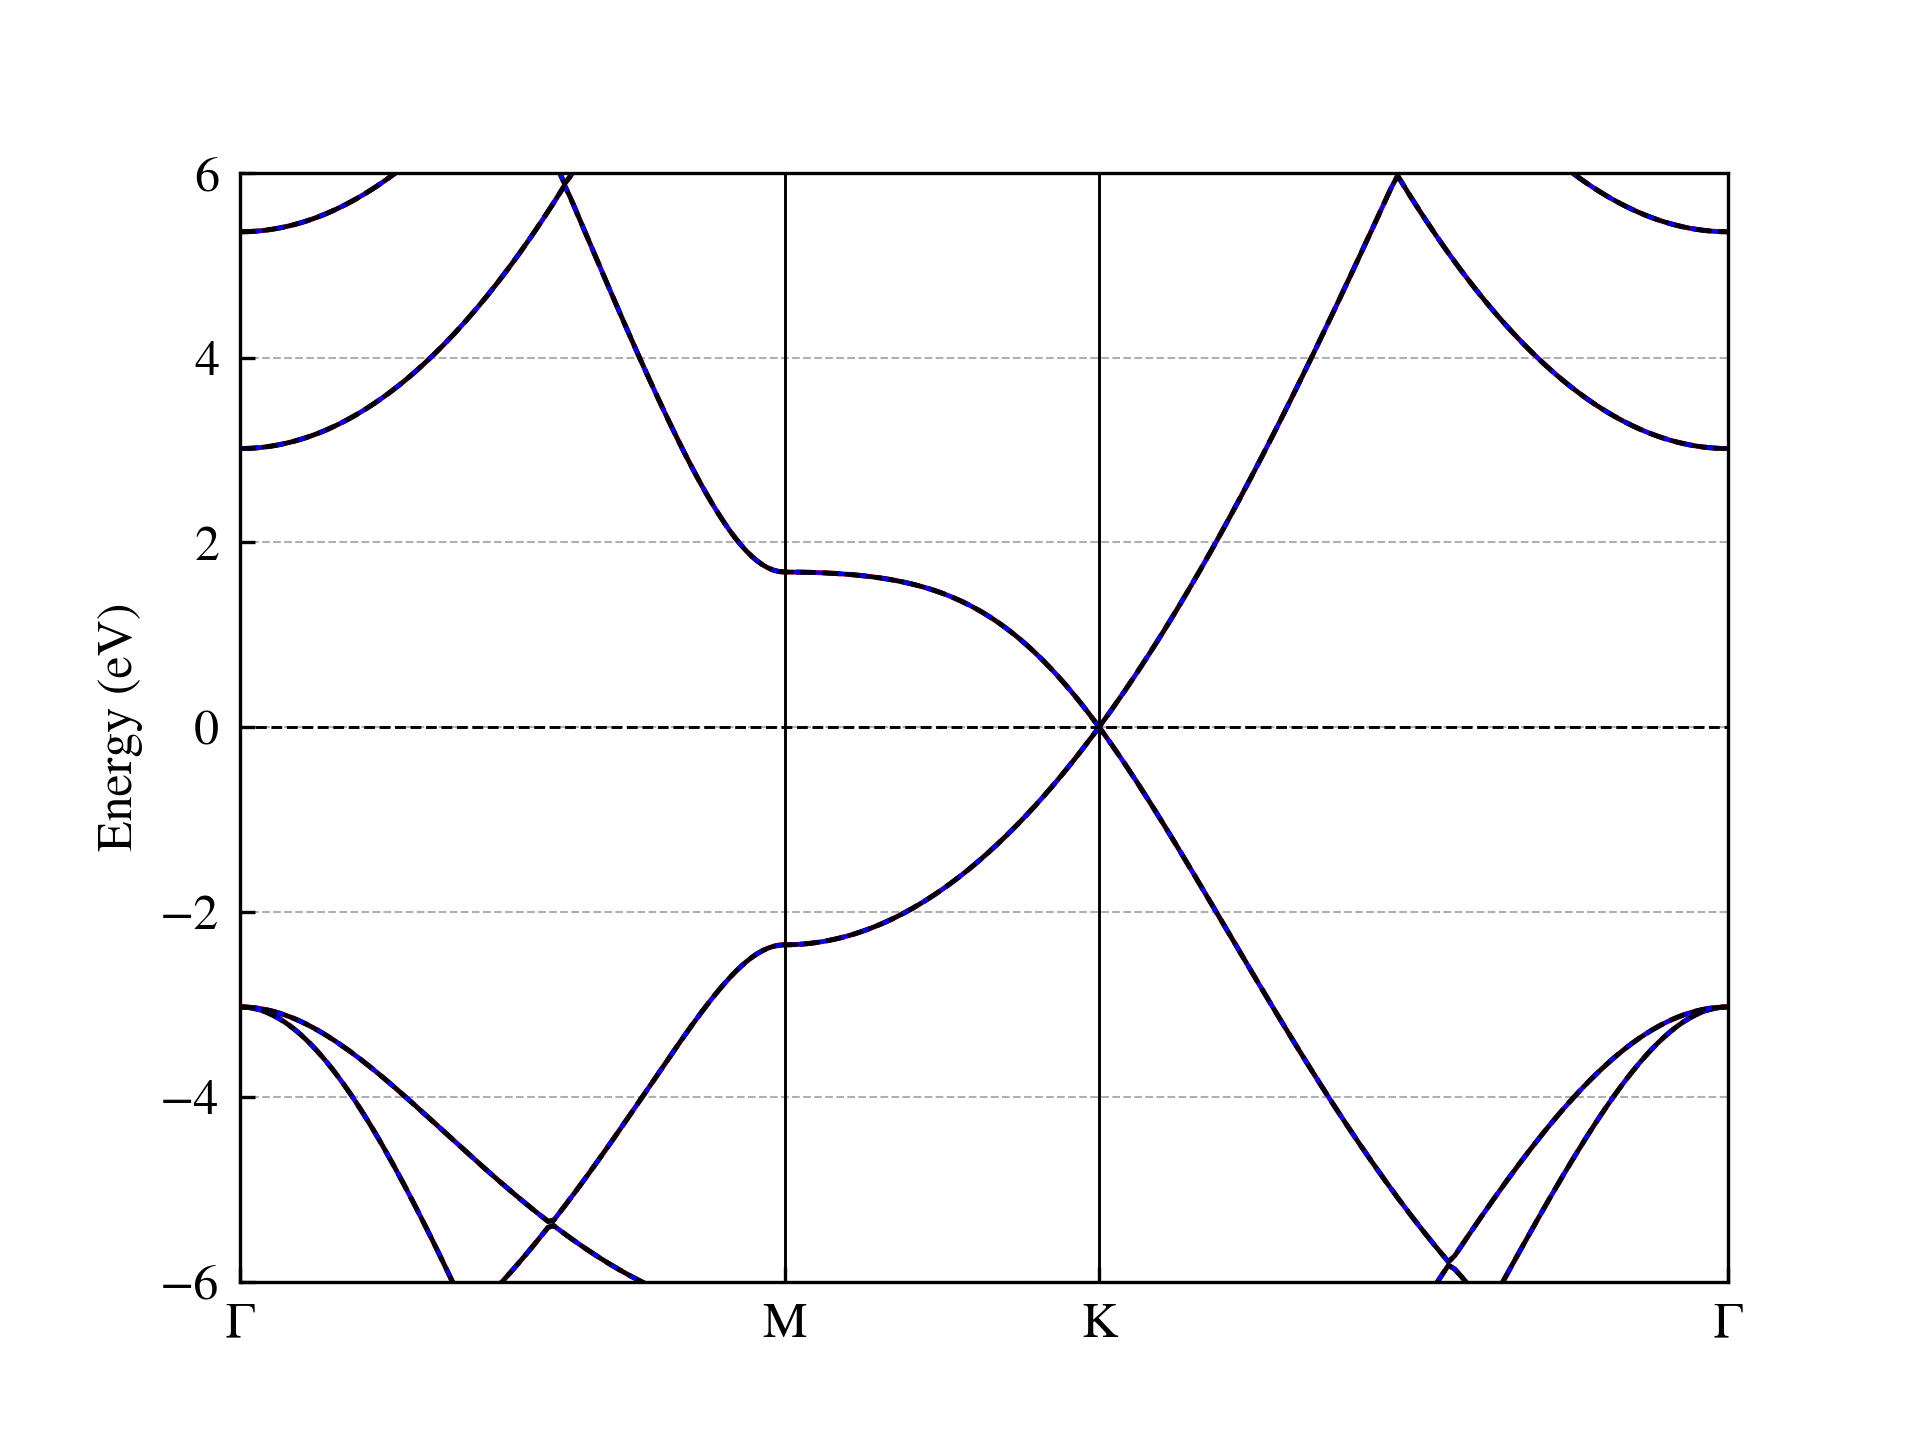
\includegraphics[width=0.9\textwidth]{../figure/Graphene-cl.band.png}}
  \subfigure[DOS compare]{
    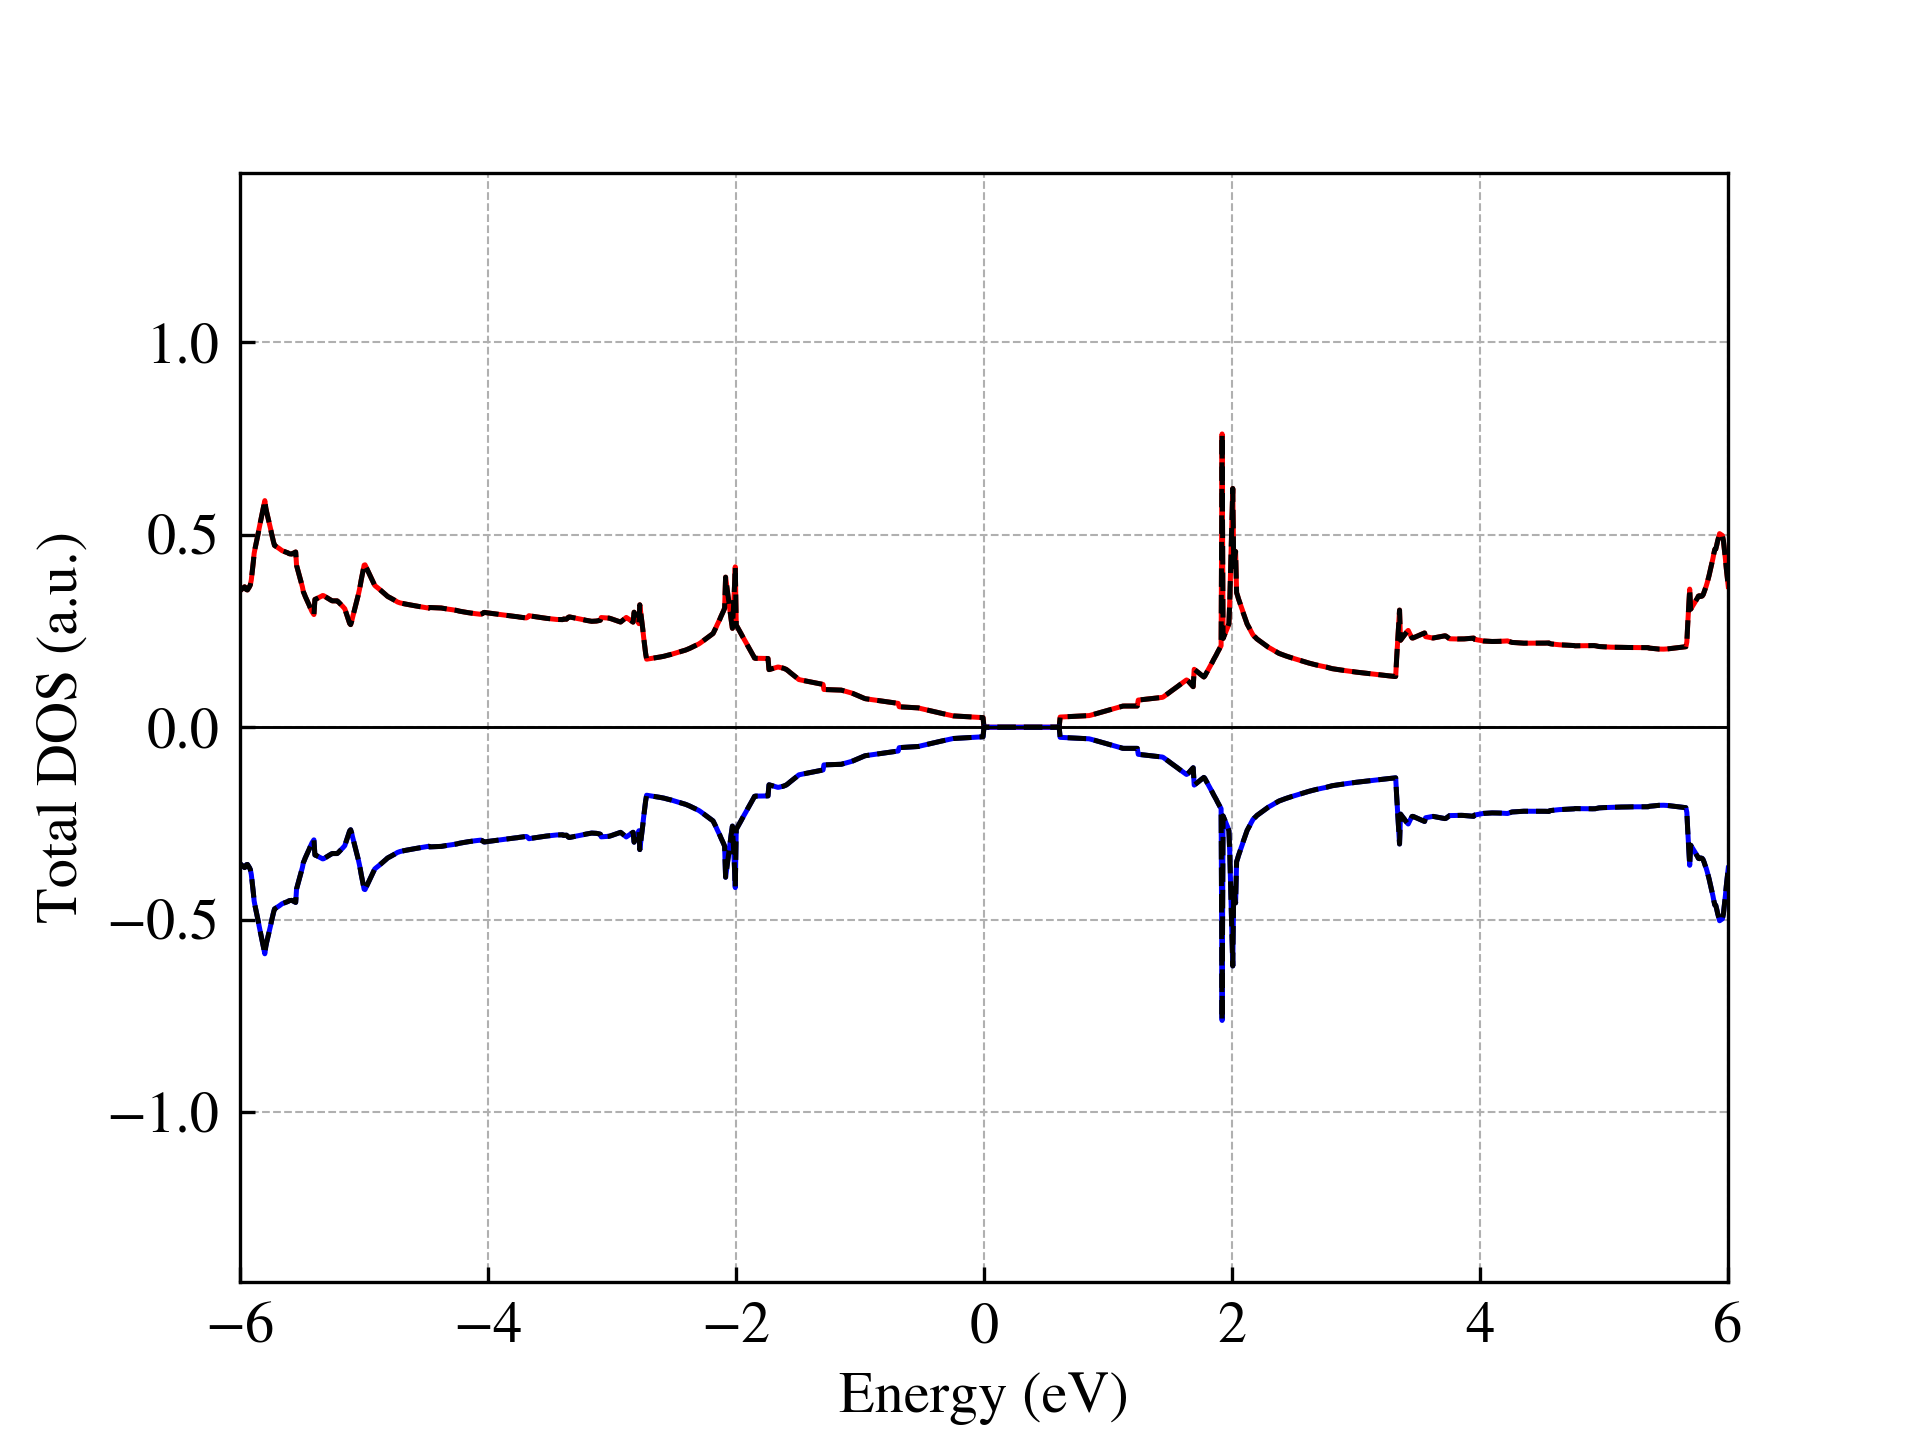
\includegraphics[width=0.9\textwidth]{../figure/Graphene-cl.dos.png}}
  \caption{Band-DOS compare}
  \label{fig::banddos::1}
\end{figure}
 
 
\end{document}
